\documentclass{article}

\setlength{\textheight}{25.7cm}
\setlength{\textwidth}{16cm}
\setlength{\unitlength}{1mm}
\setlength{\topskip}{2.5truecm}
\topmargin 260mm \advance \topmargin -\textheight 
\divide \topmargin by 2 \advance \topmargin -1in 
\headheight 0pt \headsep 0pt \leftmargin 210mm \advance
\leftmargin -\textwidth 
\divide \leftmargin by 2 \advance \leftmargin -1in 
\oddsidemargin \leftmargin \evensidemargin \leftmargin
\parindent=0pt

\frenchspacing

\usepackage[english]{babel}
\usepackage{amsmath}
\usepackage{float}
\usepackage{graphicx}
\usepackage{subcaption}
\restylefloat{table}

\usepackage{listings}
\lstset{language=C++, showstringspaces=false, basicstyle=\small,
  numbers=left, numberstyle=\tiny, numberfirstline=false,
  stepnumber=1, tabsize=4, 
  commentstyle=\ttfamily, identifierstyle=\ttfamily,
  stringstyle=\itshape}

\title{Neural Networks: Assignment 2}
\author{Pepijn van Heiningen \\ \texttt{pvheinin@liacs.nl} \and Michiel Vos \\ \texttt{msvos@liacs.nl}}

\begin{document}

\maketitle

\section{Introduction}
The second assignment of the Neural Networks course consits of three tasks:\\
\begin{itemize}
\item Task 1: Function Optimization
\item Task 2: The XOR Problem
\item Task 3: Handwritten digit recognition
\end{itemize}

For the first task, we were given the Rosenbrock's function, and we were asked to test 5 different algorithms for finding the global minimum of this function. The purpose is to get an insight into the limitations of the classical gradient descent algorithm. 

%Task 2

%Task 3

\newpage
\section{Task 1: Function Optimization}
\subsection{Problem Description}
The Rosenbrock function is a function that is used as a performance test for optimization algorithms. The equation can be found in figure \ref{eq:rosen}. It has a global minimum at the point (1,1), where the value of $f = 0$. This is visualized in figure \ref{fig:rosenbrock}. \\

\begin{figure}[H]
\[f(x,y) = 100 * (y-x^2)^2 + (1 - x)^2\]
\caption{The Rosenbrock's function}
\label{eq:rosen}
\end{figure}

We were given the task to optimize the Rosenbrock function using five different algorithms, and subsequently compare their performance, in order to get an insight into the advantages, disadvantages and limitations of the different algorithms.\\

\begin{figure}[H]
	\centering
		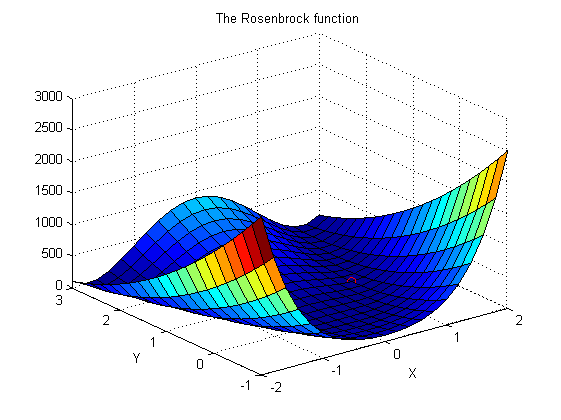
\includegraphics[scale=0.8]{rosenbrock.png}
	\caption{The Rosenbrock function, with minimal point}
	\label{fig:rosenbrock}
\end{figure}

The 5 different algorithms we tested are:
\begin{itemize}
\item Gradient descent
\item Gradient descent with line search
\item Scaled conjugate gradient
\item Conjugate gradient
\item Quasi-Newton
\end{itemize}

To get a good comparison between the algorithms, each algorithm was run 100 times.
We first generated 100 random points around (-1,1) as starting points. Each algorithm was started from the same random point.\\

\newpage
There were 4 different measures to compare the algorithms with:
\begin{itemize}
\item The average number of evaluations of $f$
\item The average number of evaluations of the gradient of $f$
\item The average run time of the algorithm
\item The average ``success rate''. 
\end{itemize}

Together these measures should provide a decent indication which algorithm performs better. Because some functions might be a lot more computationally expensive to evaluate than the Rosenbrock function, the number of evaluations of both the function and the gradient should be as low as possible. A run obviously shouldn't take too long, and it should have a high success rate. \\

The success rate is measured as reaching the minimum with an accuracy of 0.0001. This means that when the optimal point found by the algorithm is evaluated, the value of $f$ is smaller than 0.0001. Of course we would like to have an optimizer that gets a 100\% accuracy every time the algorithm is ran, but that is not always possible. 

\subsection{Implementation}
In figure \ref{fig:code} you can see the pseudo-code of the implemented algorithm.

\begin{figure}[h]
\begin{verbatim}
    starting_point = repmat([-1,1],100,1) + 0.5*randn(100,2);
    options = foptions;         % Standard options
    options(1) = -1;            % Turn off printing completely
    options(3) = 1e-8;          % Tolerance in value of function
    options(14) = 100;          % Max. 100 iterations of algorithm
    options(18) = 0.001;        % Learning rate    
    default_options = options;		
    functionList = {@graddesc, @graddesc, @scg, @conjgrad, @quasinew};
    for i = 1:100
        for j = 1:5
            options = default_options;
            if(j==1 || j==2)
                options(18) = 0.008;
            end
            if(j==2)
                options(7) = 1;
            end
            tic;
            [dump, options, dump, dump] = functionList{j}('rosen', starting_point(i,:), options, 'rosegrad');
            time = toc;
            results(i,j,1) = options(10);
            results(i,j,2) = options(11);
            results(i,j,3) = time;
            results(i,j,4) = options(8);
        end 
    end  
\end{verbatim}
\caption{Pseudo-code of task 1.}
\label{fig:code}
\end{figure}

As described in the assignment, we run the algorithms using 100 randomly generated starting points from the distribution \texttt{[-1, 1] + 0.5 * randn(1,2)}. 

We set the options of the algorithm to the default options, with a few changes, we set the tolerance of the function value to $1*10^{-8}$, the iterations to 100, and we use a different learning rate for the two gradient descent algorithms. The reasoning behind the value is described in section \ref{sec:experiments}.
%Partial derivatives of f

In figure \ref{fig:partdiv}, we show the partial derivatives of the Rosenbrock function.
\begin{figure}[H]
\[\frac{\rho f}{\rho x} = 400x^3 + 2x - 400*yx - 2\]
\[\frac{\rho f}{\rho y} = 200y - 200*x^2\]
\caption{Partial derivatives of $f$}
\label{fig:partdiv}
\end{figure}

\subsection{Experiments}
\label{sec:experiments}
%Gradient descent experiments
In task $1.3$ we were asked to tune both gradient descent algorithms manually. We first kept the number of iterations to 100, and tested different values of the learing rate.

\begin{table*}[H]
	\centering
		\begin{tabular}{l|l|l}
		Learning rate & Gradient Descent & Gradient Descent with linesearch \\
		\hline
		0.05 & 0 & 0.054 \\
		0.01 & 0 & 0.058 \\
		0.008 & 0 & 0.058 \\
		0.005 & 0 & 0.056 \\
		0.001 & 0 & 0.038 \\
		0.0001 & 0 & 0.052 \\
		0.00001 & 0 & 0.050 \\
		\end{tabular}
\end{table*}
    
The values are averages over 500 runs. We then tested the best value on 100 runs with 100.000 iterations, and the gradient descent algorithm with line search reached an accuracy of 100\%. The standard gradient descent still got 0\%.
As you can see the optimal error is somewhere around a learning rate of 0.008, which is why we set the learning rate for the experiment to that value.

In order to acquire additional insights into how the algorithms work, we plotted the optimal points found after each iteration in the following plot.

\begin{figure}[H]
	\centering
	\begin{subfigure}[b]{0.45\textwidth}
		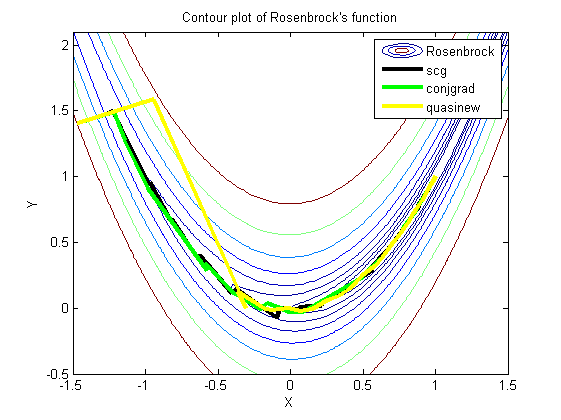
\includegraphics[width=\textwidth]{rosenbrocktask1.png}
		\caption{Nadenken}
		\label{fig:rosenbrocktask1}
	\end{subfigure}
	\begin{subfigure}[b]{0.45\textwidth}
		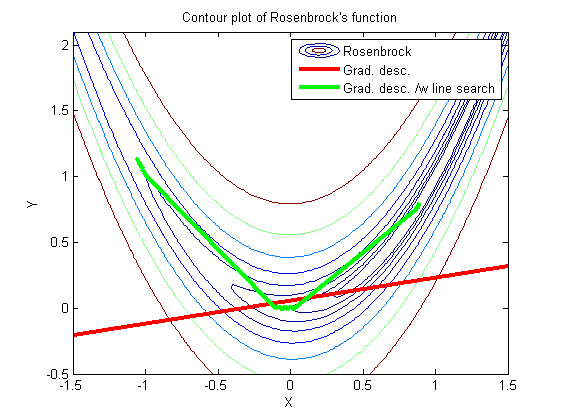
\includegraphics[width=\textwidth]{rosenbrocktask12.png}
		\caption{Nadenken}
		\label{fig:rosenbrocktask1}
	\end{subfigure}	
\end{figure}

\begin{table}[H]
	\centering
	\begin{tabular}{| l | l | l | l | l |}
		\hline
		Function                        & Evaluation  & Gradient evaluation & Runtime & Successrate \\ \hline
		Gradient descent                & 101         & 100  & 0.00778          & 0\% \\ \hline
		Gradient descent /w line search & 1816.93     & 98   & 0.19121          & 6\% \\ \hline
		Scaled conjugate gradient       & 0.47        & 0.7  & $5.376*10^{-5}$  & 100\% \\ \hline
		Conjugate gradients             & 3.64        & 0.25 & 0.0003924        & 100\% \\ \hline
		Quasi-Newton                    & 0.69        & 0.22 & $7.9669*10^{-5}$  & 100\% \\ \hline
	\end{tabular}
	\caption{Results of the 5 algorithms. All values are averages.}
	\label{table:results}
\end{table}

In table \ref{table:results} you can find the results of the different algorithms. All 5 algorithms were run on an Intel Core i5-3470, the values are averages over 100 runs. The parameters used for the algorithms are described in the section `Implementation'. As you can see the gradient descent algorithm, even after optimization, still achieves a successrate of 0\% on the data. We took a look at the output-coordinates of the algorithm, and it shows that this setting of the learning rate is too high, because the coordinates keep growing until they reach infinity. Gradient descent with line search already works a lot better, but it costs more function evaluations. The other three methods clearly achieve better results on all fronts, with less evaluations, a shorter runtime and higher successrates.

\subsection{Conclusions}
%Which algorithm is best? Which is worst?
%What is the expected number of function evaluations (including evaluations of gradients)
%needed to reach the optimum? What might be the reason for the very poor performance
%of the gradient descent algorithm?
The best algorithm is hard to tell. Both the Scaled Conjugate Gradient approach and the Quasi-Newton algorithm perform well on this particular problem. The Scaled Conjugate Gradient uses less function evaluations than Quasi-Newton, but Quasi-Newton uses less gradient evaluations. The runtime of both algorithms is almost equal, and they both achieve a successrate of 100\%. It depends on the computational difficulty of the problem which algorithms is better. If a function evaluation is costly, SCG might be the better approach, but if gradient evaluations are expensive, Quasi-Newton might be better. The expected number of function evaluations is probably around 1 for both SCG and Quasi-Newton
The worst algorithm is clearly gradient descent, since it doesn't find good solutions, even in 100 runs there are no successful solutions. Gradient descent with line search is the slowest algorithm of them all, but because it does produce some useful solutions it is better than the original gradient descent algorithm.
The reason for the very poor performance of the gradient descent algorithm is probably that if the learing rate is set too high, the algorithms best coordinates will `explode' into infinity. If the learning rate is set to a lower rate, 100 iterations are not enough to get to the optimal point. Because the Rosenberg function has such a narrow valley, finding the optimal value is very difficult.

\newpage
\section{Task 2: The XOR Problem}
\subsection{Problem Description}

\subsection{Implementation}

\subsection{Experiments}

\subsection{Conclusions}

\newpage
\section{Task 3: Handwritten Digit Recognition with MLP}
%The purpose of this task is to compare the accuracy of MLP networks to the single layer
%networks that you’ve investigated in Assignment 1. Train several MLP networks with the
%number of hidden nodes ranging between 1 and 100 (not all!) and 10 output nodes. Chose
%a suitable number of hidden nodes experimentally and a training method that is sufficiently
%fast. Try three possible activation functions for the output nodes: linear, logistic and
%softmax (study the code of mlp.m to get more details). To make sure that you understand
%what is optimized during the training process, study the function mlperr.m to find out which
%error measures correspond to the three activation functions. Write down in your report the
%definitions (formulas) of these error measures.
%Summarize the results of your experiments in a table. What setup was most successful?
%What classification rate have you achieved?
In task 3 we had to compare the Multilayer Perceptron networks to the single layer networks we've investigated in Assignment 1.

\subsection{Problem Description}
We were given the handwritten digits dataset from Assignment 1 again, and were now asked to implement a multilayer perceptron network, and train it to recognize handwritten digits.
The goal is of course to achieve the highest classification rate posssible.

\subsection{Implementation}
%Pseudocode


\subsection{Experiments}
We first tried to find the best number of hidden nodes. In the plot of \ref{fig:hidden_nodes} you can see that the softmax activation function yields the best results. We set the number of training iterations to 100 as a first try, and used the Scaled Conjugate Gradient as a training method. 

\begin{figure}[H]
	\centering
		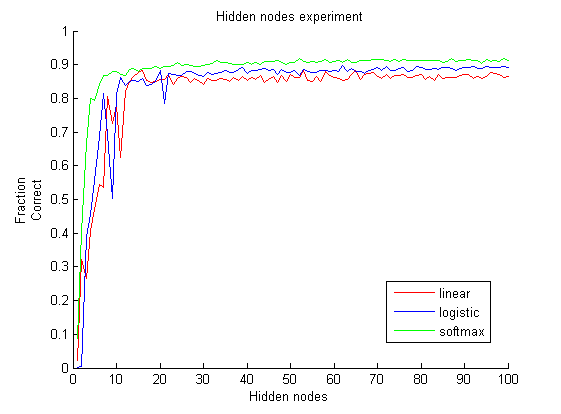
\includegraphics[width=\textwidth]{hidden_nodes.png}
    \caption{Nadenken}
    \label{fig:hidden_nodes}
\end{figure}

To check whether there are differences between the Scaled Conjugate Gradient method, Quasi-Newton and Backpropagation, we show the classification rates and runtime in table ...

Finally we used cross-validation to train the network to get the optimal classification rate.

\subsubsection{Activation functions}
\begin{figure}[H]
	\centering
%	edata = 0.5*sum(sum((y - t).^2));
	\begin{eqnarray}
		error & = & y - t \\
		error & = & t * log(y) + (1 - t) * log(1 - y) \\
		error & = & t * log(y)
	\end{eqnarray}
	\caption{Error measurements in multiple activation functions. (1) Logistic (2) Logistic (3) Softmax }
\end{figure}

\subsection{Conclusions}
As you can see in section ... blabla



\end{document}
